\section{Toepassingen van VAM op kwantum- en kernprocessen}
\label{sec:LENR_QED}
\subsection*{LENR via resonantietunneling}

Zwaartekrachtsverval door vorticiteit verlaagt tijdelijk de Coulomb-barrière:

\begin{equation}
    V_\text{Coulomb} = \frac{Z_1 Z_2 e^2}{4\pi \varepsilon_0 r}, \quad \Delta P = \frac{1}{2} \rho_\text{\ae} r_c^2 (\Omega_1^2 + \Omega_2^2)
\end{equation}

Resonantie treedt op wanneer:

\begin{equation}
    \Delta P \geq \frac{Z_1 Z_2 e^2}{4\pi \varepsilon_0 r_t^2}
\end{equation}

\subsection*{Resonante Ætherische tunneling en LENR in VAM}

In het Vortex Æther Model (VAM) worden laagenergetische kernreacties (LENR) geherinterpreteerd als resonante tunnelinggebeurtenissen die worden gemedieerd door gestructureerde wervelinteracties in de Æther. In tegenstelling tot conventionele kwantumtunneling, die afhankelijk is van deeltjesgolffuncties die een statische Coulomb-potentiaalbarrière penetreren, stelt VAM dat lokale drukminima – voortkomend uit wervel-geïnduceerde Bernoulli-tekorten – de barrière tijdelijk kunnen verminderen of volledig kunnen elimineren~\cite{Barcelo2011,Volovik2003}.

De klassieke Coulomb-afstoting tussen twee kernen van ladingen \( Z_1 e \) en \( Z_2 e \) wordt gegeven door:
\begin{equation}
    V_\text{Coulomb}(r) = \frac{Z_1 Z_2 e^2}{4\pi \varepsilon_0 r}
\end{equation}

In VAM genereren twee roterende wervelknopen in de nabijheid van \( r \sim 2r_c \) een door werveling geïnduceerde drukval~\cite{Saffman1992} via:
\begin{equation}
    \Delta P = \frac{1}{2} \rho_\text{\ae} r_c^2 (\Omega_1^2 + \Omega_2^2)
\end{equation}

Deze drukval wijzigt de effectieve interactiepotentiaal:
\begin{equation}
    V_\text{eff}(r) = V_\text{Coulomb}(r) - \Phi_\omega(r)
\end{equation}
waarbij de wervelpotentiaal \( \Phi_\omega(r) \) wordt gedefinieerd door:
\begin{equation}
    \Phi_\omega(r) = \gamma \int \frac{|\vec{\omega}(r')|^2}{|\vec{r} - \vec{r}'|} \, d^3r',
    \quad \text{met} \quad
    \gamma = G \rho_\text{\ae}^2
\end{equation}

Resonante tunneling treedt op wanneer het gecombineerde effect van \( \Delta P \) en \( \Phi_\omega \) de Coulombbarrière bij een kritische scheiding \( r_t \) neutraliseert:
\begin{equation}
    \frac{1}{2} \rho_\text{\ae} r_c^2 (\Omega_1^2 + \Omega_2^2) \geq \frac{Z_1 Z_2 e^2}{4\pi \varepsilon_0 r_t^2}
\end{equation}

De resulterende conditie maakt overgangen mogelijk, zelfs bij thermische of subthermische kinetische energieën, waardoor LENR-processen kunnen plaatsvinden zonder de barrière daadwerkelijk te hoeven overwinnen. In plaats daarvan wordt deze dynamisch uitgewist via wervelresonantie – een mechanisme dat consistent is met sommige empirische observaties~\cite{Storms2021}. De tunneling is dus een manifestatie van Ætherische fase-uitlijning en drukgemedieerde coherentie in beperkte wervelconfiguraties.



\subsection*{VAM Quantum Electrodynamics (QED) Lagrangian}

In het Vortex Æther Model (VAM) ontstaat de interactie tussen wervelknopen en elektromagnetische velden uit hun helicoïdale structuur en de daarmee gepaarde geïnduceerde vectorpotentialen. De standaard Lagrangiaan van de kwantumelektrodynamica (QED) wordt in dit model vervangen door:

\begin{equation}
    \mathcal{L}_\text{VAM-QED} =
    \bar{\psi} \left[ i \gamma^\mu \partial_\mu
                   - \gamma^\mu \left( \frac{C_e^2 r_c}{\lambda_c} \right) A_\mu
                   - \left( \frac{8\pi \rho_\text{\ae} r_c^3 Lk}{C_e} \right) \right] \psi
    - \frac{1}{4} F_{\mu\nu} F^{\mu\nu}
\end{equation}

In deze formulering:

\begin{itemize}
    \item Ontstaat de massa als gevolg van topologisch verbonden wervelkernen, waarbij de heliciteit van de wervelstructuur de rol van massa speelt~\cite{Volovik2003}.
    \item Komt de ijkkoppeling voort uit æthercirculatie en het daaruit voortvloeiende vectorpotentiaal.
    \item Blijft de elektromagnetische veldtensor \( F_{\mu\nu} \) ongewijzigd, die de rotatie van de æther (de krulcomponent) beschrijft in de omringende superfluïde.
\end{itemize}

Deze alternatieve Lagrangiaan koppelt dus wervelstructuren direct aan veldinteracties, waarbij de gebruikelijke constanten \( m \) (massa) en \( q \) (lading) worden vervangen door emergente termen die voortkomen uit de geometrie, rotatiesnelheid en topologie van het æthermedium.

Door afleiding van de Euler–Lagrangevergelijking voor het spinorveld \( \psi \), vinden we:

\begin{equation}
    \boxed{ \left( i \gamma^\mu \partial_\mu - \gamma^\mu q_\text{vortex} A_\mu - M_\text{vortex} \right)\psi = 0 }
\end{equation}

Deze vergelijking is structureel identiek aan de Dirac-vergelijking, maar met fysische parameters die voortkomen uit wervelmechanica in plaats van als fundamenteel gegeven. Daarmee levert VAM een alternatief voor de oorsprong van massa en lading~\cite{Barcelo2011,Volovik2003}.

\begin{figure}[H]
    \centering
    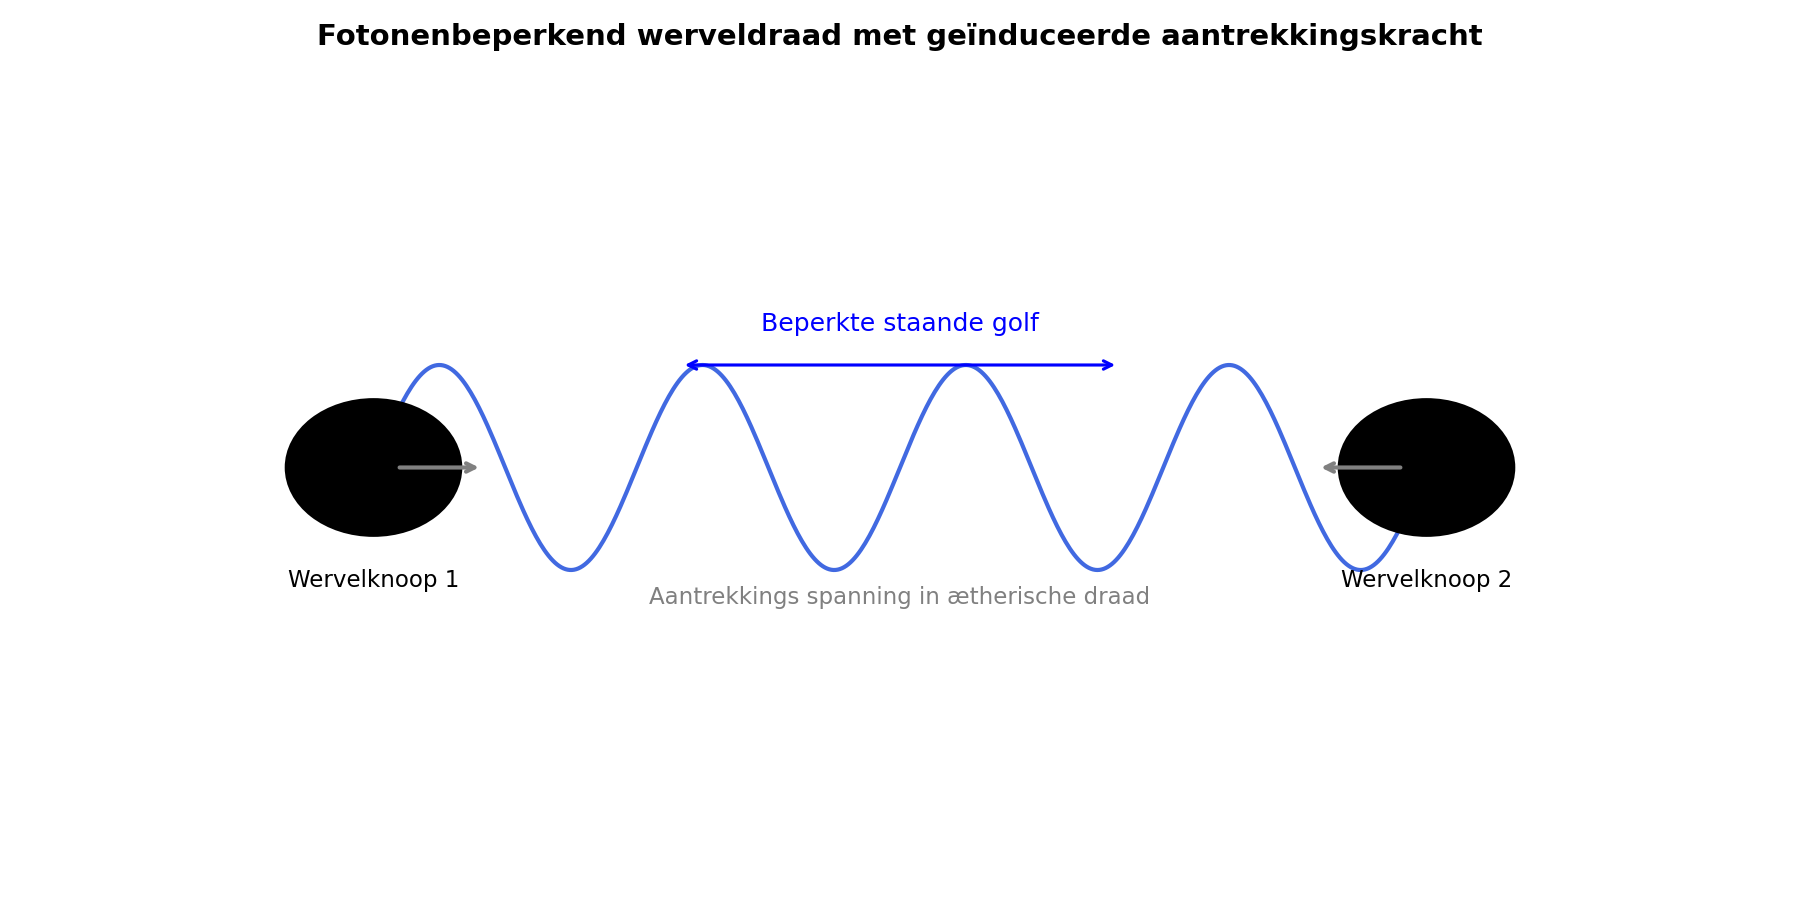
\includegraphics[width=0.85\textwidth]{images/08-Photon-ConfiningVortexThreadGravitation_nl}
    \caption{Fotonenopsluiting en -geleiding langs werveldraden in de ether. Dit visualiseert de VAM-interpretatie van elektromagnetische voortplanting, waarbij het foton gelokaliseerde trajectbuiging en resonantie vertoont rond gestructureerde wervellijnen. De opsluiting ontstaat op natuurlijke wijze door topologische drukminima en circulerende etherstroming, waardoor de abstracte veldrepresentatie wordt vervangen door een tastbaar wervelkanaal.}
    \label{fig:photon_confine}
\end{figure}